%=====================================================================
\section{A first mathematical certificate (RQ2)}\label{sec:certificate}
%=====================================================================
Simulation can only test the starting states we try. A \emph{certificate} is a mathematical proof, checked by a computer, that every state in some set recovers. In this report the certificates are proven for the \emph{linearized} model with thrust limits; how well they carry over to the nonlinear drone is measured by simulation, not proven. RQ2 needs such a set: the \emph{capture set} of the failure controller. If we can show that every state the drone can reach during the undetected phase lies inside the capture set, recovery is guaranteed. This section builds a first capture set (experiment E5) and measures how conservative it is.

\subsection{The idea: an energy-like function that always decreases}
Take the closed loop of the failure LQR on the 10-state linear model, written in deviations from the equilibrium. Without limits it would be $\dot{\vect x} = (A - BK)\vect x$. With the thrust limits it is
\begin{equation}
  \dot{\vect x} = A\vect x + B\operatorname{sat}(F\vect x), \qquad F = -K,
\end{equation}
where $\operatorname{sat}$ clips each input deviation to $[-\bar u_i, \bar u_i]$. Consider the quadratic function $V(\vect x) = \vect x^\top P\vect x$ with $P$ positive definite, and the ellipsoid $\mathcal E = \{\vect x : V(\vect x)\le1\}$. If $V$ decreases along every trajectory that starts in $\mathcal E$, no trajectory can leave $\mathcal E$, and all of them go to the equilibrium. Then $\mathcal E$ is a certified capture set. The question is how to find $P$, and how to handle the clipping, which makes the system nonlinear.

\begin{plain}
Picture a bowl whose bottom is the equilibrium. If we can prove that the drone's state always moves downhill in the bowl, then any state that starts below a certain rim stays below it and slides to the bottom. The certificate is the bowl ($P$) and the rim (the ellipsoid). The thrust limits make the drone weaker when it is far from the bottom, so the rim cannot be arbitrarily high.
\end{plain}

\subsection{Handling the thrust limits (Hu and Lin)}
Hu and Lin~\cite{hu2001saturation} give a sufficient condition based on the following observation. Choose a second, auxiliary gain $H$. If the state is in the region where $|H_i\vect x|\le\bar u_i$ for every input $i$, then the clipped input $\operatorname{sat}(F\vect x)$ is always some mixture (a convex combination) of the vectors
\begin{equation}
  D F\vect x + (I - D)H\vect x, \qquad D \in\mathcal D,
\end{equation}
where $\mathcal D$ is the set of diagonal matrices with 0 or 1 on the diagonal ($2^3 = 8$ of them for three inputs). Each $D$ picks, input by input, either the real gain $F$ or the auxiliary gain $H$. So if $V$ decreases for each of these 8 \emph{linear} systems, it also decreases for the clipped one, inside the region where $|H_i\vect x|\le\bar u_i$.

\subsection{Turning it into LMIs}
For one vertex, ``$V$ decreases at rate at least $2\mu V$'' means
\begin{equation}
  \big(A + B(DF + D^-H)\big)^\top P + P\big(A + B(DF + D^-H)\big) + 2\mu P \preceq 0, \qquad D^- = I - D .
\end{equation}
This contains the product of the unknowns $P$ and $H$, so it is not linear. The standard fix is a change of variables: multiply from both sides by $Q = P^{-1}$ and write $Y = HQ$. The condition becomes
\begin{equation}\label{eq:lmi1}
  AQ + QA^\top + B\big(DFQ + D^-Y\big) + \big(DFQ + D^-Y\big)^\top B^\top + 2\mu Q \preceq -\epsilon I \qquad \forall D\in\mathcal D,
\end{equation}
which is linear in the unknowns $Q$ and $Y$: a linear matrix inequality (we add a small margin $\epsilon$ for numerical safety). The ellipsoid must also lie inside the region where the trick is valid. The largest value of $|H_i\vect x|$ on $\mathcal E$ is $\sqrt{H_iQH_i^\top}$, so we need $H_iQH_i^\top \le \bar u_i^2$, which by a Schur complement is the LMI
\begin{equation}\label{eq:lmi2}
  \begin{pmatrix} \bar u_i^2 & Y_i \\ Y_i^\top & Q \end{pmatrix} \succeq 0, \qquad i = 1, 2, 3 .
\end{equation}
($Y_i$ is row $i$ of $Y$.) Finally, we want the ellipsoid to be large in the direction we care about: from the equilibrium towards $\vect x_{\text{on}}$, the state right after a failure in hover (zero body rates, level attitude, motors at $mg/4$). ``$\beta\vect x_{\text{on}}$ lies in $\mathcal E$'' means $\beta^2\,\vect x_{\text{on}}^\top Q^{-1}\vect x_{\text{on}}\le1$; with $t = 1/\beta^2$ this is again a Schur complement,
\begin{equation}
  \begin{pmatrix} t & \vect x_{\text{on}}^\top \\ \vect x_{\text{on}} & Q\end{pmatrix}\succeq 0,
\end{equation}
and we minimize $t$, which maximizes $\beta$. A value $\beta\ge1$ would mean the failure state itself is certified. (To get a ``general-purpose'' ellipsoid instead, we maximize its volume, $\log\det Q$, under the same constraints.)

Two practical details. The plant's thrust limits are not symmetric around the trim (rotor 2 is at 1.02\,N, between 0.2 and 3.8\,N), but the trick needs symmetric levels, so we take the smaller distance to either limit: $\bar{\vect u} = (1.76, 0.82, 1.76)$\,N; a certificate with these levels also holds for the real limits. And the motor-state deviations must stay within their physical range, so we add $Q_{ii}\le\bar u_i^2$ for the three motor states. Without this bound the problem is badly conditioned: the open-loop model is only marginally stable, and the solver ``certifies'' an almost unbounded, physically meaningless set (tilt deviations above 1, motor deviations above 100\,N).

\begin{codebox}{the certificate in CVXPY}
\begin{lstlisting}
Q = cp.Variable((n, n), symmetric=True);  Y = cp.Variable((m, n))
cons = [Q >> eps * np.eye(n)]
for bits in itertools.product([0, 1], repeat=m):          # the 2^m vertices D
    D = np.diag(bits); Dm = np.eye(m) - D
    M = D @ F @ Q + Dm @ Y
    L = A @ Q + Q @ A.T + B @ M + (B @ M).T + 2 * decay * Q
    cons.append(0.5 * (L + L.T) << -eps * np.eye(n))     # LMI (lmi1)
for i in range(m):
    row = cp.reshape(Y[i, :], (1, n), order="C")
    cons.append(cp.bmat([[np.array([[ubar[i] ** 2]]), row], [row.T, Q]]) >> 0)  # (lmi2)
for i, b in enumerate(box):                               # motor states in range
    if np.isfinite(b): cons.append(Q[i, i] <= b ** 2)
t = cp.Variable()
cons.append(cp.bmat([[cp.reshape(t, (1, 1), order="C"), d.T], [d, Q]]) >> 0)
cp.Problem(cp.Minimize(t), cons).solve(solver="CLARABEL")  # beta = 1/sqrt(t)
\end{lstlisting}
\end{codebox}
The problems are modelled with CVXPY~\cite{diamond2016cvxpy} and solved with the interior-point solver Clarabel~\cite{goulart2024clarabel}, with SCS~\cite{odonoghue2016scs} as a fallback. A test samples 500 points on the boundary of a computed ellipsoid and checks that $V$ really decreases there with the true clipping.

\subsection{Results}
\begin{table}[h]
\centering\small
\caption{Certified ellipsoids for several required decay rates $\mu$. The half-widths are those of the largest-volume ellipsoid (maximizing $\log\det Q$); $\beta$ comes from a second problem that maximizes the extent towards the failure state. $^{*}$Solver status ``optimal\_inaccurate'' (solved to lower accuracy).}\label{tab:cert}
\begin{tabular}{cccccc}
\toprule
$\mu$ (1/s) & $\Delta p, \Delta q, \Delta r$ (rad/s) & $\Delta n_x, \Delta n_y$ & $\Delta z$ (m) & $\beta$ \\
\midrule
0.0$^{*}$ & 2.23, 3.49, 6.20 & 0.42, 0.36 & 3.17 & 0.223 \\
0.1 & 2.17, 3.49, 6.09 & 0.41, 0.35 & 2.99 & 0.221 \\
0.3 & 2.07, 3.50, 5.89 & 0.40, 0.34 & 2.61 & 0.218 \\
0.5 & 1.96, 3.52, 5.76 & 0.38, 0.32 & 2.17 & 0.215 \\
\bottomrule
\end{tabular}
\end{table}

\paragraph{Certified versus simulated.} The certificate covers $\beta\approx0.22$ of the way from the equilibrium to the failure state (Table~\ref{tab:cert}); asking for a faster decay shrinks it only slightly. To see how conservative this is, we started the nonlinear simulation at $\beta\vect x_{\text{on}}$ for $\beta = 0.1, 0.2, \dots, 1.0$ with the failure LQR and no delay. Every start up to $\beta = 0.7$ recovered without turning over (height loss 0.42\,m at 0.7); at 0.8 and 0.9 the attitude was captured but the drone turned over, and at 1.0 it was not captured. So the certificate is about three times conservative in this direction, and this LQR on its own cannot recover safely from the failure state itself, which is why the spin-up phase is needed.

\paragraph{Where the controller fails.} We also simulated a $21\times21$ grid of starting points in the plane of yaw-rate deviation $\Delta r$ and tilt deviation $\Delta n_y$, all other states at equilibrium (Figure~\ref{fig:cert}). 376 of 441 points recovered without turning over; 7\% of these lie inside the certified slice, the rest is the conservatism gap. All failures occur at spin rates of 4.8\,rad/s or less, and none at 6.8\,rad/s or more. In other words, the LQR works well as long as the drone already spins reasonably fast, and fails when it starts from a slow spin, which is exactly the situation right after a failure. A certificate built from one linearization at the full spin (19\,rad/s) cannot reach that region.

\begin{figure}[h]
\centering
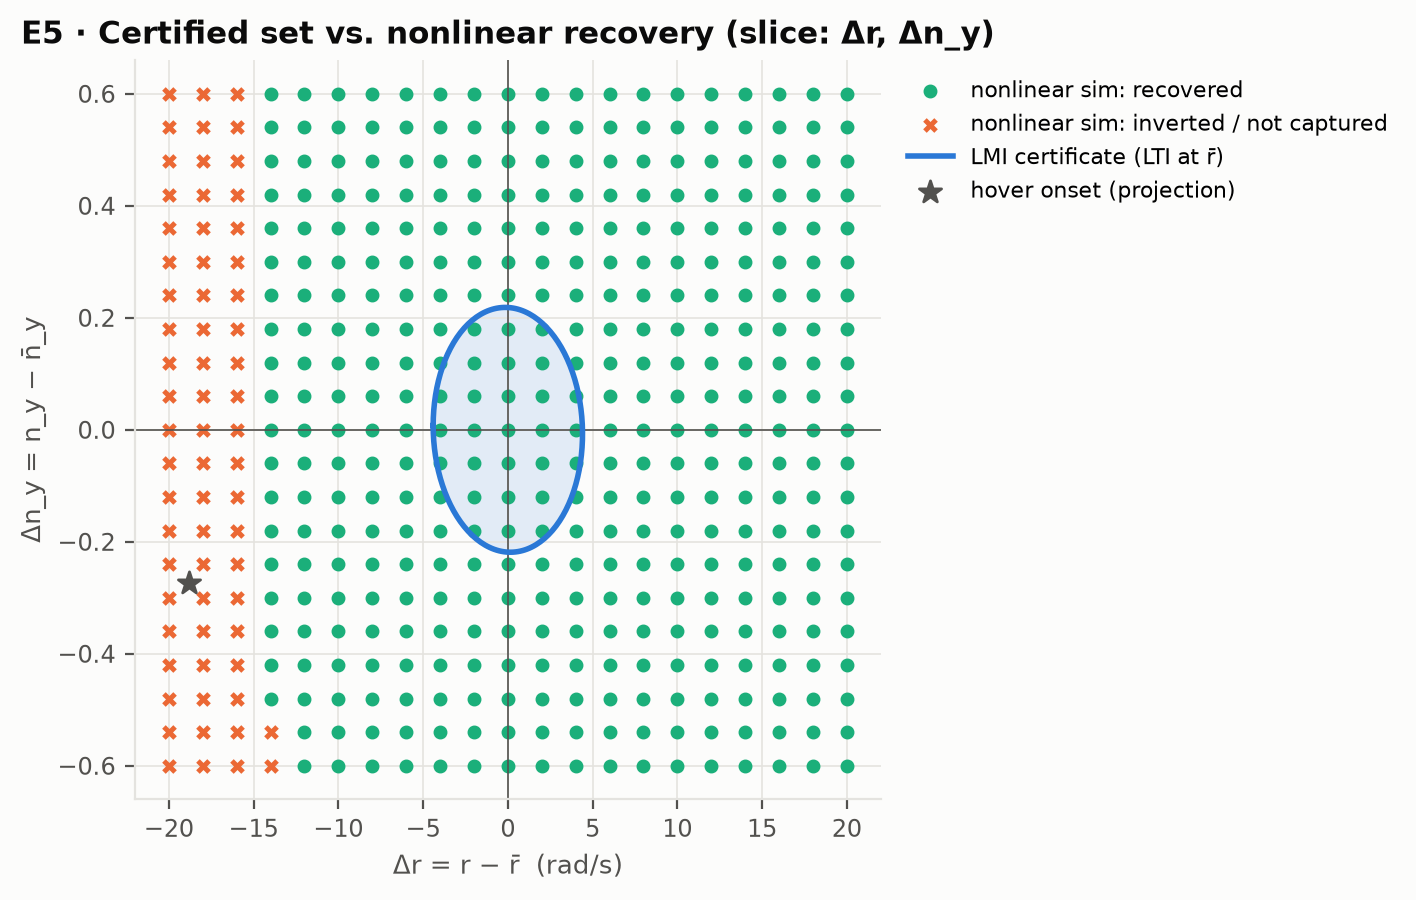
\includegraphics[width=0.75\linewidth]{figures/e5_certificate_slice.png}
\caption{Slice $(\Delta r, \Delta n_y)$ of the certified ellipsoid ($\mu = 0.1$\,s$^{-1}$) against a grid of nonlinear simulations. Dots: recovered; crosses: turned over or not captured; star: projection of the failure state (labelled ``hover onset'' in the plot). ``LTI at $\bar r$'' means the certificate uses the linear model at the equilibrium yaw rate.}\label{fig:cert}
\end{figure}

\subsection{From here to a certified delay budget (planned)}
The results point to the next steps, which are not implemented yet:
\begin{enumerate}
  \item \textbf{A certificate over the whole spin-up.} If the other operating-point values are held fixed, the linearized matrix depends affinely on the yaw rate $r$ (otherwise they become additional scheduling parameters, and linearizing away from an equilibrium adds a drift term). Treating $r$ as a parameter in an interval $[r_{\text{onset}}, \bar r + \delta]$ and requiring the LMIs~\eqref{eq:lmi1} at the two ends with a common $Q$ (a linear parameter-varying, LPV, certificate) would certify the whole interval. LPV synthesis on the yaw rate~\cite{stephan2018lpv} and recoverable sets at the relaxed hover~\cite{qi2016recoverable} exist; our aim is to use such a set as the capture target of a delay budget.
  \item \textbf{The reachable set of the undetected phase.} During the delay the drone obeys an \emph{affine} linear model (linear plus a constant term) $\dot{\vect x} = A_f\vect x + \vect d$ (healthy controller, rotor 4 missing; $\vect d$ is the constant push from the missing thrust). Starting from an ellipsoid $\mathcal X_0$ of pre-failure states, the states reachable at time $\tau$ form the shifted ellipsoid $\mathcal R(\tau) = e^{A_f\tau}\mathcal X_0 \oplus \{\int_0^\tau e^{A_f s}\vect d\,ds\}$, where $\oplus$ (the Minkowski sum) adds the fixed shift to every point of the set.
  \item \textbf{The certified delay.} $\tau^\star = \sup\{\tau : M\mathcal R(\tau)\subseteq\mathcal C\}$, where $M$ maps healthy-flight states to failure-controller coordinates and $\mathcal C$ is the capture set. Containment of one ellipsoid in another can be written as an LMI by the S-procedure (a standard way to turn ``one quadratic inequality implies another'' into a matrix inequality), and $\tau^\star$ is found by bisection.
\end{enumerate}
The main risk is that a single quadratic function over the whole spin-up is infeasible or too conservative; the fallbacks are a parameter-dependent Lyapunov function, or a chain of nested ellipsoids along the spin-up.
